\chapter{Introducción específica} % Main chapter title

\label{Chapter2}

%----------------------------------------------------------------------------------------
%	SECTION 1
%----------------------------------------------------------------------------------------
En este capítulo se  realiza un revisión detallada de los dispositivos y tecnologías utilizados y que fueron desarrollados por terceros para comprender las decisiones de diseño tomadas que se mencionan en el capítulo \ref{Chapter3}. 

%----------------------------------------------------------------------------------------
\section{Electrodos de pH}
\label{sec:electrodoPH}

Un electrodo muy usado hoy en día, es el electrodo combinado que está formado por dos electrodos dentro del mismo encapsulado. En la figura \ref{fig:electrodoCombinado} se observa un electrodo combinado que está formado por un electrodo de referencia, que consiste en un alambre clorurado de plata en una solución de KCl saturada, y un electrodo indicador, formado por el alambre clorurado de plata más una membrana de vidrio sensible al pH.

\begin{figure}[htbp]
	\centering
	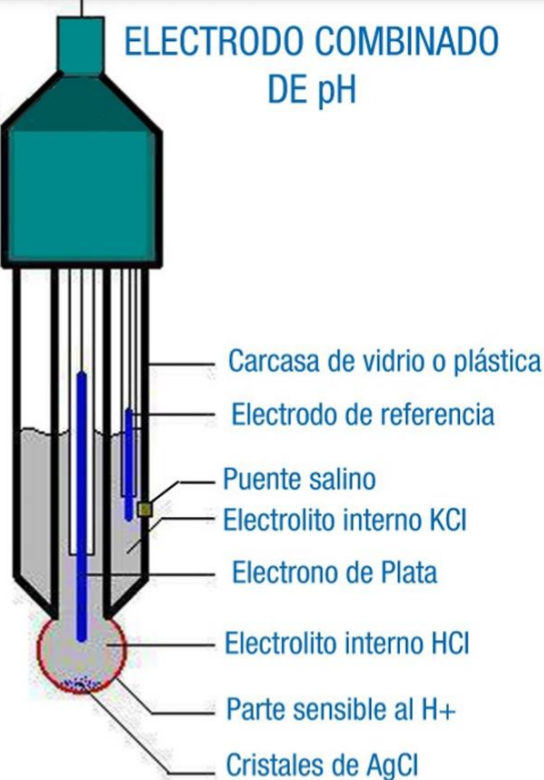
\includegraphics[width=.5\textwidth]{./Figures/electrodoCombinado.png}
	\caption{Electrodo combinado de pH de Ag/AgCl\protect\footnotemark.}
	\label{fig:electrodoCombinado}
\end{figure}

\footnotetext{Imagen tomada de \url{http://depa.fquim.unam.mx/amyd/archivero/ELECTRODOSDEMEDIDAYDEREFERENCIA_22645.pdf}}

El potencial de un electrodo está dado por la ecuación de Nernst, que se puede escribir de manera simplificada como muestra la ecuación \ref{eq:Nernst} .

\begin{equation}
	\label{eq:Nernst}
E = E_{0} + k pH
\end{equation}
\citep{ARTICLE:4}

donde E es el potencial corregido del electrodo, $E_{0}$ es el potencial en condiciones estándar (valores tabulados), k una variable que depende de la temperatura y pH es el valor de pH de la muestra.

En este trabajo se utilizó el electrodo comercial marca HANNA HI-1230B de la figura \ref{fig:hi-1230b}, definido por el área de Ingeniería Química, ya que permite realizar titulaciones potenciométricas ácido-base para detectar nitrógeno en suelo y alcalinidad en agua. Específicamente, este electrodo es de plata sumergido en una disolución de cloruro de potasio que se ha saturado con cloruro de plata, y presenta un potencial de 0 mV para un valor de pH de 7,01, y una pendiente de -0,0174pH/mV. En base a estos datos se puede crear la recta que relaciona la potencial del electrodo con el valor de pH y que está dada por la ecuación \ref{eq:phElectrodo}:

\begin{equation}
	\label{eq:phElectrodo}
pH = -0,0174 E + 7,01
\end{equation}

donde E es el potencial entregado por el electrodo y pH es el valor correspondiente de pH de la muestra a 25 °C. Para una muestra con ph 0 la salida del electrodo es de 402,8 mV y para una muestra de ph 14 el potencial es de -401,7 mV.

\begin{figure}[htbp]
	\centering
	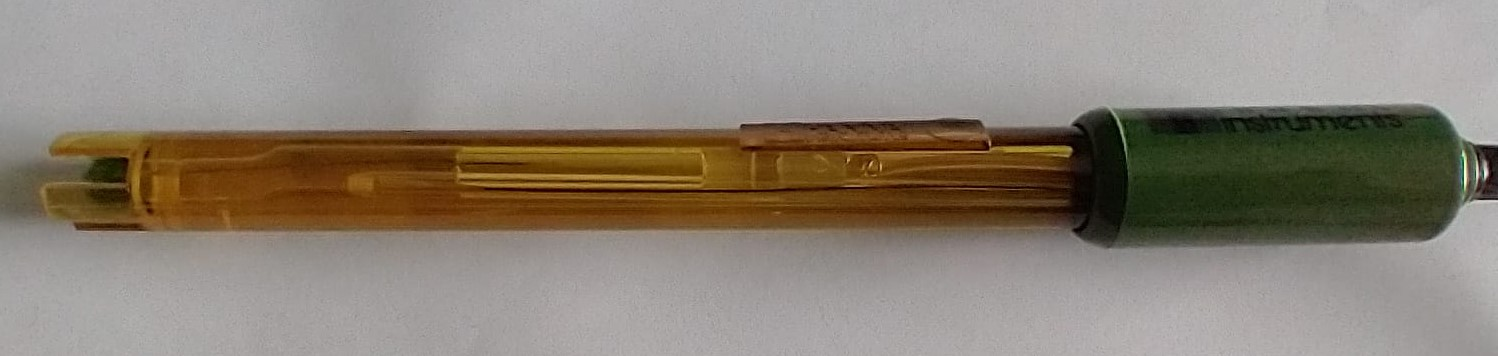
\includegraphics[width=.6\textwidth]{./Figures/hi-1230b.jpeg}
	\caption{Electrodo HI-1230B.}
	\label{fig:hi-1230b}
\end{figure}

%----------------------------------------------------------------------------------------
\section{Bombas peristálticas}
\label{sec:bomba}

Una bomba peristáltica es un tipo de bomba hidráulica que se emplea para transportar diferentes tipos de líquidos, y generalmente es usada cuando se emplean fluidos limpios o estériles ya que el mecanismo de la bomba no los contamina al desplazarlos \citep{ARTICLE:5}. Está formada por una manguera flexible situada dentro de la cubierta de la bomba, que puede ser circular o lineal, y un rotor compuesto por varios rodillos que comprimen la manguera, tal y como se muestra en la figura \ref{fig:bombaPeristEsq}. Cuando el rotor gira, se genera un vacío que hace que el líquido ingrese y fluya por la manguera.

\begin{figure}[htbp]
	\centering
	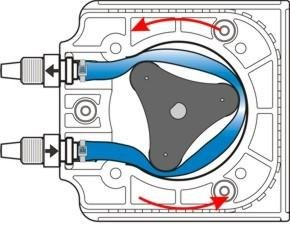
\includegraphics[width=.4\textwidth]{./Figures/bombaPeristEsq.png}
	\caption{Bomba peristáltica\protect\footnotemark.}
	\label{fig:bombaPeristEsq}
\end{figure}

\footnotetext{Imagen tomada de \url{https://www.researchgate.net/figure/Figura-3-Principio-de-funcionamiento-de-una-bomba-peristaltica-de-3-rodillos_fig2_275959587}}


Para este trabajo se utilizó la bomba desarrollada por el área de electromecánica, que hace uso de un motor paso a paso bipolar Nema 17 marca Usongshine, como se aprecia en la figura \ref{fig:bombaAtras}.

\begin{figure}[htbp]
	\centering
	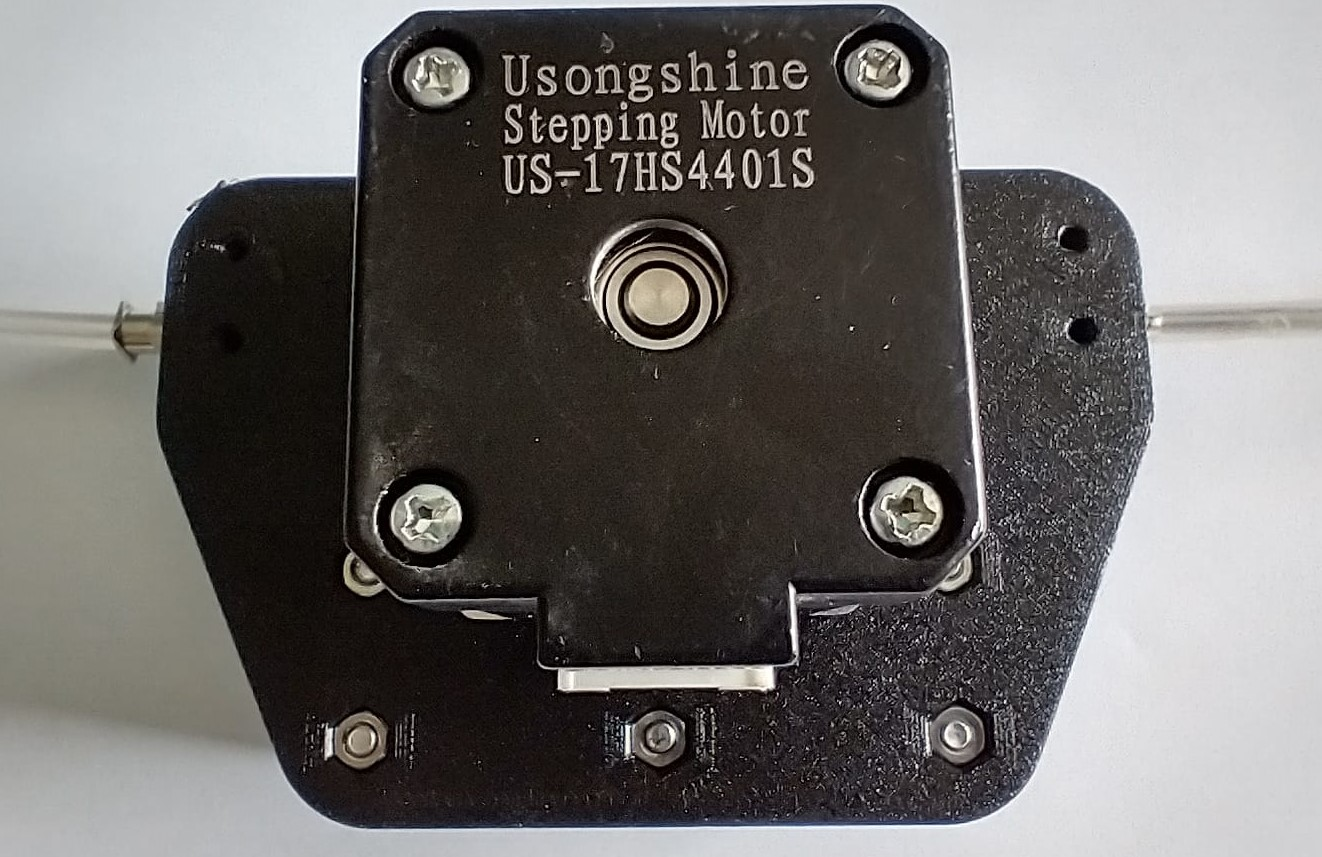
\includegraphics[width=.5\textwidth]{./Figures/bombaAtras.jpeg}
	\caption{Bomba peristáltica desarrollada por el área de Ingeniería Electromecánica. Vista del motor.}
	\label{fig:bombaAtras}
\end{figure}

La carcasa, el rotor y la cubierta exterior están impresas con ácido poliláctico (PLA) Grilon y contiene dos tipos de mangueras: una manguera PharMed BPT de 4 mm de diámetro exterior y 0,8 mm de diámetro interior que soporta las deformaciones cíclicas producidas por los rodillos del rotor, y dos mangueras genéricas de silicona para los tramos de entrada y salida. En las figura \ref{fig:bombaFrente} se observan los componentes mencionados.

\begin{figure}[htbp]
	\centering
	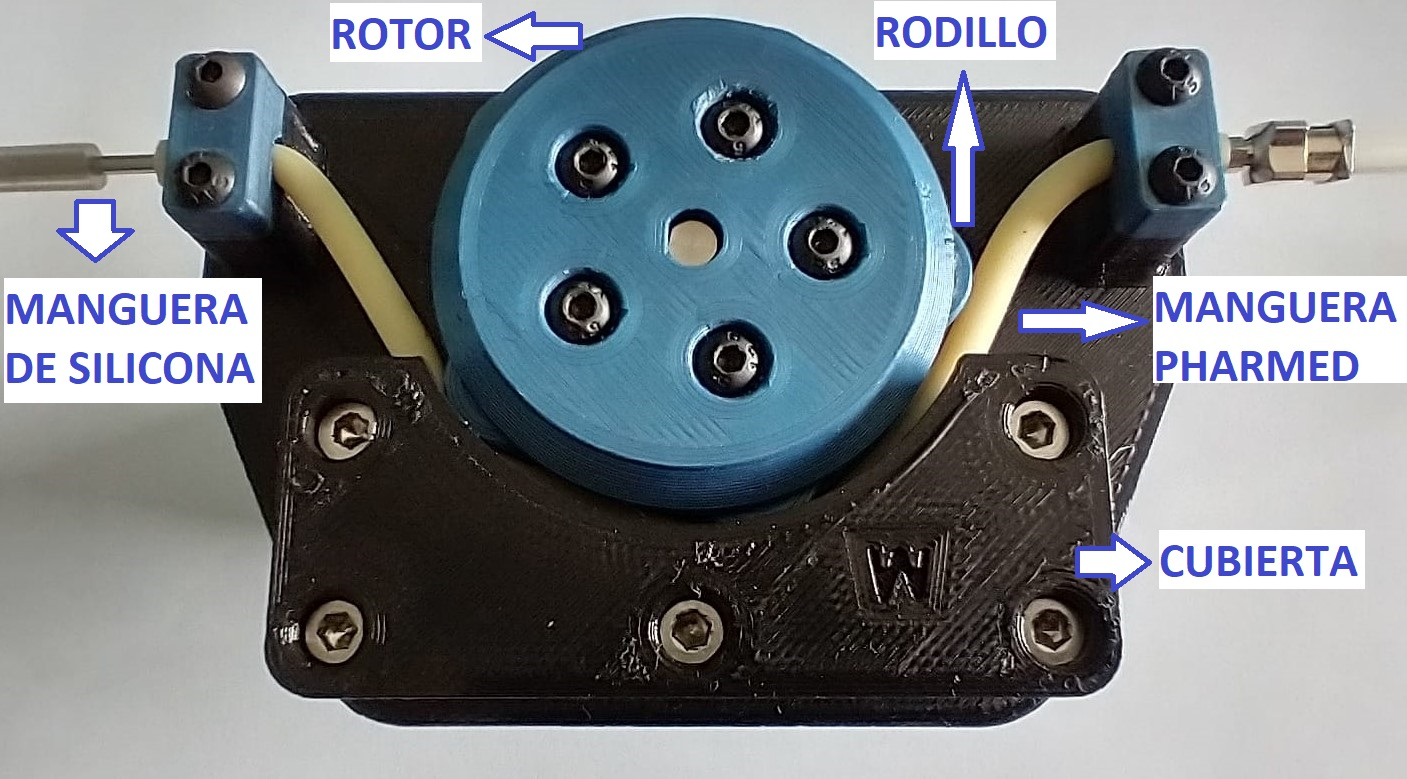
\includegraphics[width=.6\textwidth]{./Figures/bombaFrente.jpg}
	\caption{Bomba peristáltica desarrollada por el área de Ingeniería Electromecánica. Vista de los rodillos.}
	\label{fig:bombaFrente}
\end{figure}

%con un rango de voltaje apto de 5 a 36V, torque de 42 N.cm, máxima corriente 1,7A, de 1.8° por paso, lo que implica que para lograr una vuelta entera del eje (360°) el motor debe dar unos 200 pasos. 

%El diseño de las piezas mecánicas se basó en una bomba peristáltica de precisión. Para el modelado 3D se empleó el software SolidWorks®. La impresión de la carcasa, rotor y cubeta exterior se realizó con ácido poliláctico (PLA) Grilon.

%En relación con la selección de tubos flexibles o mangueras, se utilizaron dos tipos. Por un lado, una manguera PharMed BPT (de alta calidad, resistencia química, diseñada especialmente para aplicaciones de bombas peristálticas de 4 mm de diámetro exterior y 0,8 mm de diámetro interior), se empleó en la cubierta circular interior que posee la bomba y que soportará las deformaciones cíclicas producidas por los rodillos del rotor.

%Por otro lado, se utilizaron mangueras genéricas de silicona (de 4mm diámetro exterior y 0.8mm diámetro interior) para los tramos de entrada y salida de la bomba.

%----------------------------------------------------------------------------------------
\section{Otras tecnologías utilizadas}

Este trabajo se enfocó en el diseño de un prototipo de titulador, con el foco puesto en el software más que en el hardware. Es por eso que se buscaron alternativas del tipo "módulo" para los diferentes componentes, de tal forma que permita una rápida conexión del hardware y delegar la mayor parte del tiempo al desarrollo del firmware. En cada una de las siguientes secciones se describen los módulos utilizados.

\subsection{Microcontrolador ESP32}

Para el desarrollo del prototipo se utilizó la placa de desarrollo ESP32-DevKitC de la figura \ref{fig:ESP32.jpeg}. Esta placa contiene un módulo ESP32 con Wi-Fi y Bluetooth integrado y un sistema de doble núcleo, cada uno con un CPU Xtensa LX6 de 32 bit.

\begin{figure}[htbp]
	\centering
	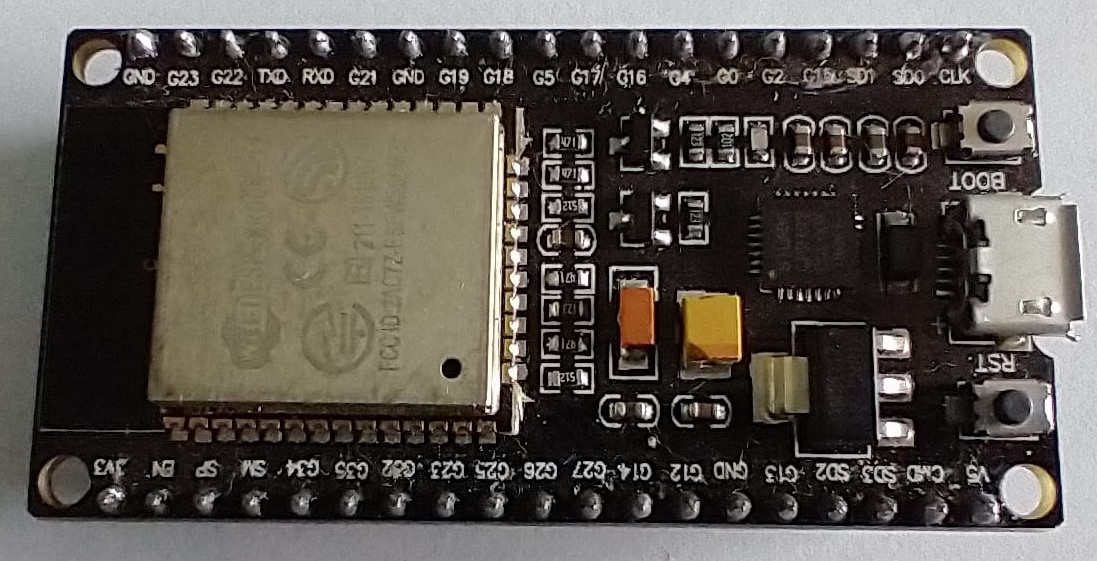
\includegraphics[width=.4\textwidth]{./Figures/ESP32.jpeg}
	\caption{Placa de desarrollo ESP32-DevKitC.}
	\label{fig:ESP32.jpeg}
\end{figure}

Las principales características de esta placa de desarrollo que se tuvieron en cuenta para el desarrollo del trabajo son las siguientes:
	\begin{itemize}
		\item Clock a 160 MHz.
		\item 4 MB de memoria flash.
		\item Wi-Fi: 802.11 b/g/n.
		\item 12-bit SAR ADC de hasta 18 canales.
		\item 3 × UART
		\item Controlador host SD
		\item PWM
	\end{itemize}

Para el desarrollo del software se utilizó el framework ESP-IDF de Espressif Systems, que ofrece una API para trabajar con una versión de FreeRTOS adaptada para aprovechar el doble núcleo del procesador, asi como también para el resto de los periféricos mencionados anteriormente.

\subsection{Pantalla táctil}

Los tituladores comerciales cuentan con una pantalla a través de la cuál se muestra una interfaz de usuario que permite acceder a las configuraciones y controlar las distintas funciones. En algunos casos la pantalla está acompañada por un teclado y en otros casos cuenta directamente con un panel táctil. Para este trabajo se decidió optar por la segunda opción ya que permite mayor flexibilidad a la hora de realizar cambios en la interfaz.

Entre las opciones disponibles en el mercado, se optó por módulo MCUFRIEND de la figura \ref{fig:LCDFrente} que contiene una pantalla LCD de 2,4" con un panel táctil y un lector de tarjetas SD.

\begin{figure}[htbp]
	\centering
	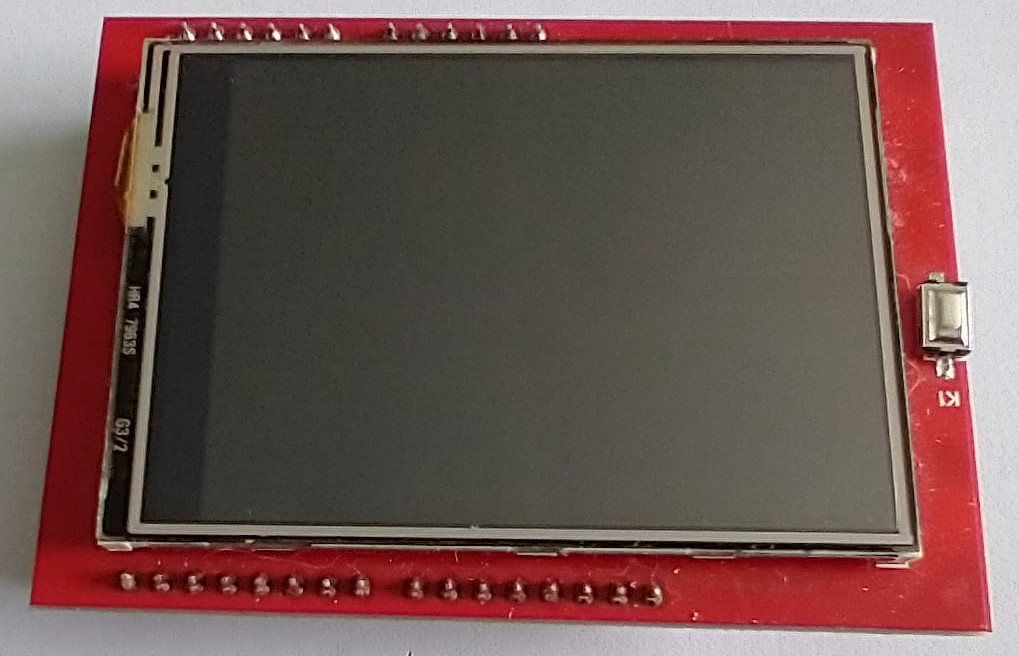
\includegraphics[width=.4\textwidth]{./Figures/LCDFrente.jpeg}
	\caption{LCD táctil MCUFRIEND.}
	\label{fig:LCDFrente}
\end{figure}

\subsection{\textit{Driver} para motor}

Previamente, en la sección \ref{sec:bomba}, se mencionó que la bomba utiliza un motor paso a paso. Para que el módulo ESP32 pueda controlarlo es necesario utilizar un \textit{driver} que otorgue los niveles de tensión y corriente necesarios para su correcto funcionamiento.

Para este trabajo se utilizó el módulo DRV8825 de la figura \ref{fig:DRV8825-Frente}, que permite el manejo de motores paso a paso de hasta 2,5 A y tiene la posibilidad de utilizar \textit{microsteping} 1/32.

\begin{figure}[htbp]
	\centering
	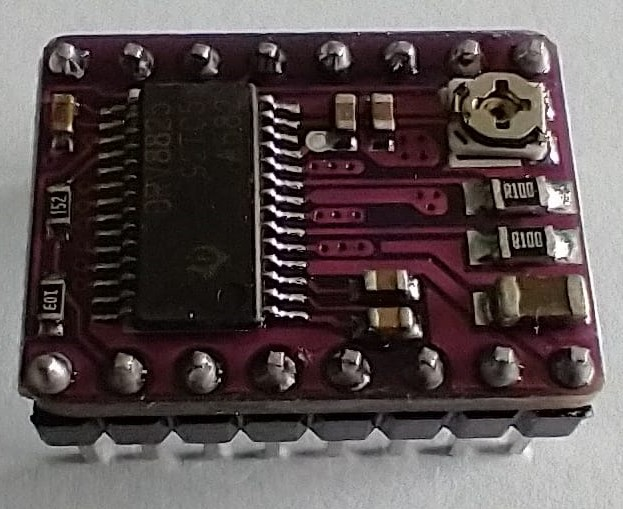
\includegraphics[width=.3\textwidth]{./Figures/DRV8825-Frente.jpeg}
	\caption{\textit{Driver} para motor paso a paso DRV8825.}
	\label{fig:DRV8825-Frente}
\end{figure}

La técnica de \textit{microsteping} permite multiplicar la cantidad de pasos que puede dar un motor para realizar una vuelta. De esta forma se puede aumentar la resolución de giro, es decir, disminuir el ángulo de paso del motor, lo que se traduce a una menor cantidad de volumen inyectada por cada paso.

\subsection{Módulo de adaptación para electrodo}

En la sección \ref{sec:electrodoPH} se mencionó que el electrodo entrega un potencial que va a depender del pH de la muestra y se ubica entre -401,7 y 402,8 mV. Para poder procesar estos valores con el ADC del ESP32, cuyo rango de entrada es de 0 a 3500 mV, es necesario adaptar esa señal para amplificar la tensión y adaptar impedancias. Para eso se utilizó el módulo pH-4502C de la figura \ref{fig:pH-4502C}.

\begin{figure}[htbp]
	\centering
	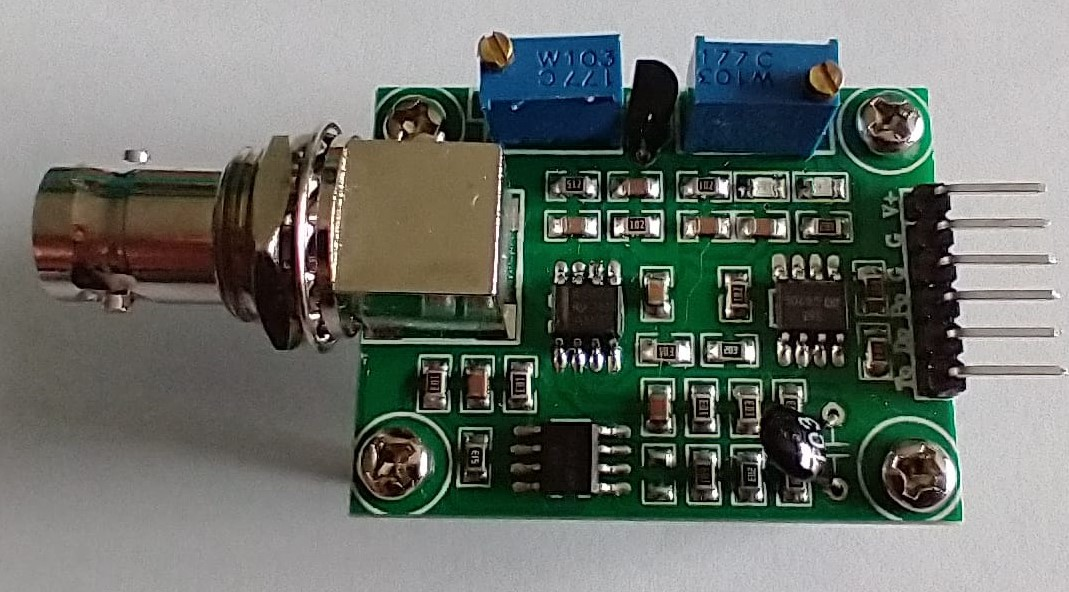
\includegraphics[width=.4\textwidth]{./Figures/pH-4502C.jpeg}
	\caption{Módulo pH-4502C.}
	\label{fig:pH-4502C}
\end{figure}

El módulo PH-4502C está formado por dos etapas. En la Fig. 4 se observa la etapa de amplificación de la señal, la cual utiliza un amplificador operacional con una configuración del tipo no inversor y con una ganancia de 2. En la Fig. 5 se muestra la etapa que permite regular la tensión de referencia. Está formado por un amplificador operacional en configuración de seguidor de tensión y un divisor resistivo con un potenciómetro que permite calibrar el nivel de tensión para evitar valores negativos en la salida del circuito.

%----------------------------------------------------------------------------------------
\section{Requerimientos}
\label{sec:requerimientos}

En esta sección se detallan los requerimientos del sistema que fueron planteados en el plan trabajo, con ligeros cambios que surgieron durante el desarrollo del trabajo.

\begin{itemize}
\item Interfaces Externas
	\begin{itemize}
	\item El hardware debe contar con una pantalla TFT táctil. [TPA-ERH-01-REQ001]
	\item El hardware debe contar con un lector de tarjetas SD. [TPA-ERH-01-REQ002]
	\item El hardware debe contar con un \textit{driver} para un motor paso a paso Nema 17. [TPA-ERH-01-REQ003]
	\item El hardware debe contar con una entrada para un electrodo de pH. [TPA-ERH-01-REQ004]
	\end{itemize}
	
\item Funciones
	\begin{itemize}
	\item El usuario debe poder elegir mediante la pantalla táctil el volumen de corte de la titulación. [TPA-ERS-01-REQ001]
	\item El usuario debe poder elegir mediante la pantalla táctil si utilizar o no el agitador. Cuando el proceso de titulación comienza, el agitador debe activarse si así lo indicó el usuario. [TPA-ERS-01-REQ002]
	\item El usuario debe poder realizar mediante la pantalla táctil el proceso de calibración con cada uno de los tres buffers. [TPA-ERS-01-REQ003]
	\item Los valores de potencial obtenidos en el proceso de la calibración se deben guardar en la memoria flash del ESP32. [TPA-ERS-01-REQ004]
	\item El valor de pH se debe calcular de manera proporcional a la recta de ajuste de los valores de potencial obtenidos en la calibración. [TPA-ERS-01-REQ005]
	\item El usuario debe poder dar inicio al proceso de titulación mediante la pantalla táctil. [TPA-ERS-01-REQ006]
	\item Durante la titulación, la pantalla debe mostrar el valor actual leído en mV y en pH y una gráfica de pH en función del tiempo. [TPA-ERS-01-REQ007]
	\item Cada valor de volumen añadido junto al valor de potencial asociado durante el proceso de titulación deben almacenarse en un archivo de texto en la tarjeta sd. No es necesario que esto se haga en tiempo real. [TPA-ERS-01-REQ008]
	\item Cada valor de volumen añadido junto al valor de potencial asociado durante el proceso de titulación deben mostrarse en una página web almacenada en la memoria flash, una vez finalizada la titulación. [TPA-ERS-01-REQ009]
	\item El usuario debe poder acceder a la página web mediante una conexión Wi-Fi. No es necesario que esto se haga en tiempo real. [TPA-ERS-01-REQ010]
	\item El sistema debe ser capaz de leer y mostrar el potencial entregado por un electrodo de pH, con una resolución de 1 mV para la lectura del potencial y de 0,01 pH para su conversión a pH. [TPA-ERS-01-REQ011]
	\item El sistema deberá inyectar una cantidad de 0,1 mL y luego esperar 5 segundos para realizar la medición de pH. La cantidad inyectada puede ser de 1 mL si el cambio de ph entre las últimas dos mediciones es menor a 0,2. [TPA-ERS-01-REQ012]
	 \item El sistema debe dejar de agregar titulante cuando se alcanza la cantidad de volumen indicada por el usuario como volumen de corte. [TPA-ERS-01-REQ013]

\end{itemize}

\item Requisitos de Rendimiento
	\begin{itemize}
	\item El sistema debe ser capaz de realizar titulaciones que involucren una cantidad máxima de 100 ml. [TPA-ERS-01-REQ014]
	\end{itemize}
	
\item Restricciones de Diseño
	\begin{itemize}
	\item Se utiliza el módulo ESP32 como computadora principal. [TPA-ERS-01-REQ015]
	\item Se utiliza la pantalla táctil MCUFRIEND 2,4'' como interfaz de usuario. [TPA-ERS-01-REQ016]
	\end{itemize}
\end{itemize}	
%----------------------------------------------------------------------------------------
% TODO LO DE ACÁ ABAJO ES EL MODELO

%\section{Estilo y convenciones}
%\label{sec:ejemplo}
%
%\subsection{Uso de mayúscula inicial para los título de secciones}
%
%Si en el texto se hace alusión a diferentes partes del trabajo referirse a ellas como capítulo, sección o subsección según corresponda. Por ejemplo: ``En el capítulo \ref{Chapter1} se explica tal cosa'', o ``En la sección \ref{sec:ejemplo} se presenta lo que sea'', o ``En la subsección \ref{subsec:ejemplo} se discute otra cosa''.
%
%Cuando se quiere poner una lista tabulada, se hace así:
%
%\begin{itemize}
%	\item Este es el primer elemento de la lista.
%	\item Este es el segundo elemento de la lista.
%\end{itemize}
%
%Notar el uso de las mayúsculas y el punto al final de cada elemento.
%
%Si se desea poner una lista numerada el formato es este:
%
%\begin{enumerate}
%	\item Este es el primer elemento de la lista.
%	\item Este es el segundo elemento de la lista.
%\end{enumerate}
%
%Notar el uso de las mayúsculas y el punto al final de cada elemento.
%
%\subsection{Este es el título de una subsección}
%\label{subsec:ejemplo}
%
%Se recomienda no utilizar \textbf{texto en negritas} en ningún párrafo, ni tampoco texto \underline{subrayado}. En cambio sí se debe utilizar \textit{texto en itálicas} para palabras en un idioma extranjero, al menos la primera vez que aparecen en el texto. En el caso de palabras que estamos inventando se deben utilizar ``comillas'', así como también para citas textuales. Por ejemplo, un \textit{digital filter} es una especie de ``selector'' que permite separar ciertos componentes armónicos en particular.
%
%La escritura debe ser impersonal. Por ejemplo, no utilizar ``el diseño del firmware lo hice de acuerdo con tal principio'', sino ``el firmware fue diseñado utilizando tal principio''. 
%
%El trabajo es algo que al momento de escribir la memoria se supone que ya está concluido, entonces todo lo que se refiera a hacer el trabajo se narra en tiempo pasado, porque es algo que ya ocurrió. Por ejemplo, "se diseñó el firmware empleando la técnica de test driven development".
%
%En cambio, la memoria es algo que está vivo cada vez que el lector la lee. Por eso transcurre siempre en tiempo presente, como por ejemplo:
%
%``En el presente capítulo se da una visión global sobre las distintas pruebas realizadas y los resultados obtenidos. Se explica el modo en que fueron llevados a cabo los test unitarios y las pruebas del sistema''.
%
%Se recomienda no utilizar una sección de glosario sino colocar la descripción de las abreviaturas como parte del mismo cuerpo del texto. Por ejemplo, RTOS (\textit{Real Time Operating System}, Sistema Operativo de Tiempo Real) o en caso de considerarlo apropiado mediante notas a pie de página.
%
%Si se desea indicar alguna página web utilizar el siguiente formato de referencias bibliográficas, dónde las referencias se detallan en la sección de bibliografía de la memoria, utilizado el formato establecido por IEEE en \citep{IEEE:citation}. Por ejemplo, ``el presente trabajo se basa en la plataforma EDU-CIAA-NXP \citep{CIAA}, la cual...''.
%
%\subsection{Figuras} 
%
%Al insertar figuras en la memoria se deben considerar determinadas pautas. Para empezar, usar siempre tipografía claramente legible. Luego, tener claro que \textbf{es incorrecto} escribir por ejemplo esto: ``El diseño elegido es un cuadrado, como se ve en la siguiente figura:''
%
%\begin{figure}[h]
%\centering
%\includegraphics[scale=.45]{./Figures/cuadradoAzul.png}
%\end{figure}
%
%La forma correcta de utilizar una figura es con referencias cruzadas, por ejemplo: ``Se eligió utilizar un cuadrado azul para el logo, como puede observarse en la figura \ref{fig:cuadradoAzul}''.
%
%\begin{figure}[ht]
%	\centering
%	\includegraphics[scale=.45]{./Figures/cuadradoAzul.png}
%	\caption{Ilustración del cuadrado azul que se eligió para el diseño del logo.}
%	\label{fig:cuadradoAzul}
%\end{figure}
%
%El texto de las figuras debe estar siempre en español, excepto que se decida reproducir una figura original tomada de alguna referencia. En ese caso la referencia de la cual se tomó la figura debe ser indicada en el epígrafe de la figura e incluida como una nota al pie, como se ilustra en la figura \ref{fig:palabraIngles}.
%
%\begin{figure}[htpb]
%	\centering
%	\includegraphics[scale=.3]{./Figures/word.jpeg}
%	\caption{Imagen tomada de la página oficial del procesador\protect\footnotemark.}
%	\label{fig:palabraIngles}
%\end{figure}
%
%\footnotetext{Imagen tomada de \url{https://goo.gl/images/i7C70w}}
%
%La figura y el epígrafe deben conformar una unidad cuyo significado principal pueda ser comprendido por el lector sin necesidad de leer el cuerpo central de la memoria. Para eso es necesario que el epígrafe sea todo lo detallado que corresponda y si en la figura se utilizan abreviaturas entonces aclarar su significado en el epígrafe o en la misma figura.
%
%
%
%\begin{figure}[ht]
%	\centering
%	\includegraphics[scale=.37]{./Figures/questionMark.png}
%	\caption{¿Por qué de pronto aparece esta figura?}
%	\label{fig:questionMark}
%\end{figure}
%
%Nunca colocar una figura en el documento antes de hacer la primera referencia a ella, como se ilustra con la figura \ref{fig:questionMark}, porque sino el lector no comprenderá por qué de pronto aparece la figura en el documento, lo que distraerá su atención.
%
%Otra posibilidad es utilizar el entorno \textit{subfigure} para incluir más de una figura, como se puede ver en la figura \ref{fig:three graphs}. Notar que se pueden referenciar también las figuras internas individualmente de esta manera: \ref{fig:1de3}, \ref{fig:2de3} y \ref{fig:3de3}.
% 
%\begin{figure}[!htpb]
%     \centering
%     \begin{subfigure}[b]{0.3\textwidth}
%         \centering
%         \includegraphics[width=.65\textwidth]{./Figures/questionMark}
%         \caption{Un caption.}
%         \label{fig:1de3}
%     \end{subfigure}
%     \hfill
%     \begin{subfigure}[b]{0.3\textwidth}
%         \centering
%         \includegraphics[width=.65\textwidth]{./Figures/questionMark}
%         \caption{Otro.}
%         \label{fig:2de3}
%     \end{subfigure}
%     \hfill
%     \begin{subfigure}[b]{0.3\textwidth}
%         \centering
%         \includegraphics[width=.65\textwidth]{./Figures/questionMark}
%         \caption{Y otro más.}
%         \label{fig:3de3}
%     \end{subfigure}
%        \caption{Tres gráficos simples}
%        \label{fig:three graphs}
%\end{figure}
%
%El código para generar las imágenes se encuentra disponible para su reutilización en el archivo \file{Chapter2.tex}.
%
%\subsection{Tablas}
%
%Para las tablas utilizar el mismo formato que para las figuras, sólo que el epígrafe se debe colocar arriba de la tabla, como se ilustra en la tabla \ref{tab:peces}. Observar que sólo algunas filas van con líneas visibles y notar el uso de las negritas para los encabezados.  La referencia se logra utilizando el comando \verb|\ref{<label>}| donde label debe estar definida dentro del entorno de la tabla.
%
%\begin{verbatim}
%\begin{table}[h]
%	\centering
%	\caption[caption corto]{caption largo más descriptivo}
%	\begin{tabular}{l c c}    
%		\toprule
%		\textbf{Especie}     & \textbf{Tamaño} & \textbf{Valor}\\
%		\midrule
%		Amphiprion Ocellaris & 10 cm           & \$ 6.000 \\		
%		Hepatus Blue Tang    & 15 cm           & \$ 7.000 \\
%		Zebrasoma Xanthurus  & 12 cm           & \$ 6.800 \\
%		\bottomrule
%		\hline
%	\end{tabular}
%	\label{tab:peces}
%\end{table}
%\end{verbatim}
%
%
%\begin{table}[h]
%	\centering
%	\caption[caption corto]{caption largo más descriptivo}
%	\begin{tabular}{l c c}    
%		\toprule
%		\textbf{Especie} 	 & \textbf{Tamaño} 		& \textbf{Valor}  \\
%		\midrule
%		Amphiprion Ocellaris & 10 cm 				& \$ 6.000 \\		
%		Hepatus Blue Tang	 & 15 cm				& \$ 7.000 \\
%		Zebrasoma Xanthurus	 & 12 cm				& \$ 6.800 \\
%		\bottomrule
%		\hline
%	\end{tabular}
%	\label{tab:peces}
%\end{table}
%
%En cada capítulo se debe reiniciar el número de conteo de las figuras y las tablas, por ejemplo, figura 2.1 o tabla 2.1, pero no se debe reiniciar el conteo en cada sección. Por suerte la plantilla se encarga de esto por nosotros.
%
%\subsection{Ecuaciones}
%\label{sec:Ecuaciones}
%
%Al insertar ecuaciones en la memoria dentro de un entorno \textit{equation}, éstas se numeran en forma automática  y se pueden referir al igual que como se hace con las figuras y tablas, por ejemplo ver la ecuación \ref{eq:metric}.
%
%\begin{equation}
%	\label{eq:metric}
%	ds^2 = c^2 dt^2 \left( \frac{d\sigma^2}{1-k\sigma^2} + \sigma^2\left[ d\theta^2 + \sin^2\theta d\phi^2 \right] \right)
%\end{equation}
%                                                        
%Es importante tener presente que si bien las ecuaciones pueden ser referidas por su número, también es correcto utilizar los dos puntos, como por ejemplo ``la expresión matemática que describe este comportamiento es la siguiente:''
%
%\begin{equation}
%	\label{eq:schrodinger}
%	\frac{\hbar^2}{2m}\nabla^2\Psi + V(\mathbf{r})\Psi = -i\hbar \frac{\partial\Psi}{\partial t}
%\end{equation}
%
%Para generar la ecuación \ref{eq:metric} se utilizó el siguiente código:
%
%\begin{verbatim}
%\begin{equation}
%	\label{eq:metric}
%	ds^2 = c^2 dt^2 \left( \frac{d\sigma^2}{1-k\sigma^2} + 
%	\sigma^2\left[ d\theta^2 + 
%	\sin^2\theta d\phi^2 \right] \right)
%\end{equation}
%\end{verbatim}
%
%Y para la ecuación \ref{eq:schrodinger}:
%
%\begin{verbatim}
%\begin{equation}
%	\label{eq:schrodinger}
%	\frac{\hbar^2}{2m}\nabla^2\Psi + V(\mathbf{r})\Psi = 
%	-i\hbar \frac{\partial\Psi}{\partial t}
%\end{equation}
%
%\end{verbatim}
